\section{Compression along a tree of windows}
\label{sec:compression-tree}

We now use Theorem~\ref{thm:predictor} to replace the old slot domains by
smaller ones.  The main issue is that a test at one window changes the
domains available at later steps.  We control each fresh test before
asking which descendants survive.  This order permits an unconditional
sum of losses and keeps the decoder independent of the old context.

\subsection{A fresh incidence test}

For points $x,y$ in opposite systems write $x\in N(y)$ when $x\perp y$.
Given a row $x_1,\ldots,x_h$ in one system, its fresh ambient test is
\begin{equation}\label{eq:fresh-test-set}
 \mathcal T(x_1,\ldots,x_h)
 =\left\{y:\sum_{j=1}^h1_{\{x_j\perp y\}}<\frac{.2h}{q}\right\}.
\end{equation}
The word ``ambient'' means that this set is defined on the entire
opposite point system, before intersection with an inherited domain.

\begin{lemma}[Validation and its conditional law]\label{lem:fresh-test}
Suppose nonempty supports $A\subseteq U_A$ and $B\subseteq U_B$ satisfy
\[
 |A||B|\ge q^5e^{-b},\qquad
 \frac{|\{(a,b')\in A\times B:a\perp b'\}|}{|A||B|}
 \le\frac{\varepsilon}{q},
\]
where $b=O(K_*)$ and $\varepsilon\le C\sigma^{-1000\beta}$.
Put $n_A=|A|$, $n_B=|B|$ and
$d_A=\log(|U_A|/n_A)$, $d_B=\log(|U_B|/n_B)$.
Suppose a decoder-known $W$ captures at least $c n_A$ points of $A$
and has size at most $n_Ae^{CP}$.

Using independent public proposal tables, one can describe two caps
$U_A'\subseteq U_A$, $U_B'\subseteq U_B$ such that
\begin{equation}\label{eq:validated-caps}
 |U_B'|\le C'q^5/n_A,\quad |U_A'|\le C'q^5/n_B,
 \qquad |B\cap U_B'|\ge .9n_B,\quad |A\cap U_A'|\ge .9n_A.
\end{equation}
The failure probability is $O(e^{-q})$, and the metadata cost is
$O(qP(d_A+d_B+1))$.
Each successful row, conditional on its past and on finding that row
before its cutoff, has density bounded by an absolute constant relative
to the true iid law of its stated hidden source.  This conditional law
does not include success of any later test or descendant.

More generally, if such a test is produced from a hidden source
contained in an original support $X$ and of size at least $c|X|$, then
for every fixed opposite point $y$,
\begin{equation}\label{eq:fresh-test-domination}
 \EE\bigl[1_{\{\text{test is produced}\}}
          1_{\{y\notin\mathcal T\}}\mid\text{prior data}\bigr]
 \le Cq\frac{|X\cap N(y)|}{|X|}.
\end{equation}
The prior data may include all original support choices and tables used
earlier, but not the current fresh table.
\end{lemma}

\begin{proof}
First consider $h_B=\lceil Cq(d_B+1)\rceil$ genuine iid draws from
$A\cap W$.  Weighted incidence variance shows that at most
$Cq^5/n_A$ points have incidence proportion less than $.5/q$ into
this source.  Each other point passes~\eqref{eq:fresh-test-set} with
probability at most $\exp(-c h_B/q)$ by Chernoff.  Since
$|U_B|=e^{d_B}n_B$ and sparsity with incidence mixing gives
$n_An_B\le Cq^5$, Markov's inequality makes the size of
$U_B\cap\mathcal T$ at most $C'q^5/n_A$ with probability at least $.99$
after choosing the constants.
The average hit proportion from this source into $B$ is at most
$C\varepsilon/q$.  Markov applied first to hit counts and then to the
fraction of $B$ rejected by the test shows that at least $.9n_B$ points
survive with probability $1-O(\varepsilon)$.  Both requirements thus
hold with probability at least $.9$.

The first cap is regarded as produced immediately after this first
acceptance, even if a later test fails.  After this first success, draw
$h_A=\lceil Cq(d_A+1)\rceil$ iid points from $B\cap U_B'$.
This is at least $.9$ of $B$, so the same argument produces
$U_A'=U_A\cap\mathcal T$ with the other two requirements.  In
particular the second cap is not intersected with $W$.

Implement the first row by proposals uniform in $W$, accepting precisely
when every entry lies in $A\cap W$ and both requirements hold.
Implement the second by proposals uniform in $U_B'$, accepting when
every entry lies in $B\cap U_B'$ and both requirements hold.
The domain/source ratios are at most $e^{CP}$: for the second use
$|U_B'|/|B\cap U_B'|\le Cq^5/(n_An_B)\le e^{CP}$.
A row of length $h$ therefore succeeds with probability at least
$.9e^{-ChP}$.  Stop after $\lceil e^{C'hP}\rceil$ proposals, for a
sufficiently large $C'$.  The failure probability is $O(e^{-q})$ and
the successful index costs $O(hP)$.

Conditioning an all-in-source row gives exactly iid draws from that
source.  Its further acceptance property has probability at least $.9$
under this iid law.  The first successful row, conditional on finding
one before the cutoff, has the same acceptance-conditioned law; its
density relative to iid is at most $1/.9$.  This proves the law assertion
and the metadata bound, including row sizes and the finite diagnostics.

Finally, conditional on being ready to produce a test, its hidden source
has at least $c|X|$ points inside $X$.  The successful-row law just proved
and the count threshold imply
\[
 \Pr(y\notin\mathcal T\mid\text{ready})
 \le Cq\frac{|X\cap N(y)|}{|X|}.
\]
Multiply by the readiness indicator and bound its probability by one.
This proves~\eqref{eq:fresh-test-domination}.  No assertion about a
descendant's later survival is used.
\end{proof}

\subsection{The tree construction and loss accounting}

The surviving window list is determined by the pre-round history and
the fresh representative indices: all its deletions use only the
numbers $\delta_i,g_i,u_i$.  Fix this list before making the independent
level choices.  Build a balanced binary tree on it from
Section~\ref{sec:compression-local}: its root is the middle window,
and recurse on the earlier and later halves.  Each node has its original
supports $A,B$ from Lemma~\ref{lem:flat-levels}.  Its inherited sets
$U_A,U_B$ initially equal the two full point systems.  At a successful
node, the left child inherits the new first-endpoint cap and the old
second-endpoint cap; the right child inherits the old first-endpoint cap
and the new second-endpoint cap.  Middle targets of the pivot window
use both new caps.  Figure~\ref{fig:pivot-tree} records these different
roles.

\begin{figure}[ht]
\centering
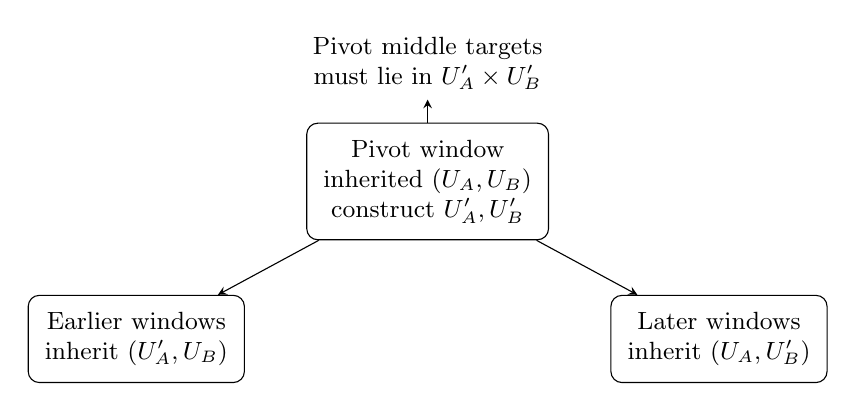
\begin{tikzpicture}[>=stealth,
 every node/.style={align=center,font=\small},
 box/.style={draw,rounded corners,inner sep=6pt}]
 \node[box] (pivot) at (0,0)
 {Pivot window\\inherited $(U_A,U_B)$\\construct $U_A',U_B'$};
 \node[box] (left) at (-3.7,-2)
 {Earlier windows\\inherit $(U_A',U_B)$};
 \node[box] (right) at (3.7,-2)
 {Later windows\\inherit $(U_A,U_B')$};
 \node (targets) at (0,1.5)
 {Pivot middle targets\\must lie in $U_A'\times U_B'$};
 \draw[->] (pivot) -- (left);
 \draw[->] (pivot) -- (right);
 \draw[->] (pivot) -- (targets);
\end{tikzpicture}
\caption{Only the endpoint facing a pivot's representative is restricted
in each descendant half.  All tests are constructed before checking
which actual middle targets they retain.}
\label{fig:pivot-tree}
\end{figure}

At a node, trim $A$ and $B$ to their inherited sets.  Drop its entire subtree
if either trim keeps fewer than $.9$ of its original support, or if the
untrimmed same-node density exceeds $\sigma^{-1000\beta}/q$.
Otherwise, the trimmed supports satisfy Theorem~\ref{thm:predictor} in
dimension four, with $b=O(K_*)$.  Apply the predictor in the orientation
of the smaller support and then Lemma~\ref{lem:fresh-test}, exchanging
the two systems if necessary.  Drop the subtree on failure.  Use
independent tables for each tree address, stage, predictor call and
validation test.

\begin{lemma}[Tree retention]\label{lem:pivot-retention}
The expected number of windows lost by this construction and the
preceding deletions is $o(w)$, where $w$ is the deterministic window
count before deletions.  Among the middle targets, the expected number
lost beyond their fixed non-middle complement is $o(k)$.
Consequently, with probability bounded below, a deterministic
$\Theta(k)$ middle targets can be retained, in order, in the two caps
of their successful pivots.
\end{lemma}

\begin{proof}
Do not inspect actual middle-target coverage while constructing the
tree.  Conditional on history, fresh representative indices and all
original support choices, apply~\eqref{eq:fresh-test-domination} to
each produced ancestor test.  Its hidden source is always a constant
fraction of the original support $X$: the node trim keeps $.9$, the
predictor captures a constant fraction, and the first validation keeps
$.9$ of the opposite trimmed support.  Predictor bias therefore does
not affect this bound.
The readiness indicator has already been removed on the right-hand side
of~\eqref{eq:fresh-test-domination}.  We may therefore sum that bound
over a descendant's original support before averaging its level choice;
we never replace that support by its law conditional on reaching the
descendant.

Average the bound over the independently chosen levels.  For every
descendant's original support, the expected fraction evicted by a
relevant ancestor fresh test is $O(\sigma^{-2000\beta})$ by
\eqref{eq:low-conflict} and Lemma~\ref{lem:flat-levels}.
Inherited sets are intersections of precisely these ambient tests.
The probability of reaching a node but failing its $.9$ trim is thus
at most a constant times the sum of these loss bounds along its path.
The same-node density rejection probability, even ignoring reach, is
$O(\sigma^{-1000\beta})$ by Markov.  Predictor and validation failures
contribute $O(e^{-cq})$ per attempted node.

The tree depth is $O(\log(w+1))=O(\log\sigma)$.
For each fixed node, summing failure bounds over its ancestor path
therefore gives $o(1)$ probability of being lost through a dropped
subtree.  Summing over nodes gives $o(w)$ expected loss.  This adds to
the $o(w)$ representative and open-band deletions already proved.

The identical fresh-test estimate applies to actual good middle targets
after integration against their endpoint marginals.  Given history and
fresh indices, these targets are independent of the auxiliary level
choices and public tables.  An earlier target faces a pivot's second
support, and a later target faces its first support, so all relevant
incidence bounds have the required temporal orientation.  At its own
pivot, the target faces both representatives.  Count bad target indices
and bad endpoints as losses.  Their total is $o(k)$ in expectation,
and the path sum bounds the remaining evictions by $o(k)$ as well.

In this argument the first pivot test is counted whenever it is
produced, without conditioning on success of the second test.
Likewise no ancestor test is conditioned on descendant survival.
Thus all the conditional-law estimates used above have the form
actually supplied by Lemma~\ref{lem:fresh-test}.
Markov now gives a positive constant probability of retaining at least
$c k$ middle targets.  Keep exactly $\lfloor c k\rfloor$ in their
original order.
\end{proof}

\subsection{The new decoder and its message length}

The encoder transmits the tree size and node statuses, successful node
constructions, and the retained slot count at each node in tree order.
The parameters $q,\eta,D,L,R,P$ and the deterministic stage budgets are
part of the common protocol.  At each successful node the message also
specifies its orientation, trimmed support sizes, row lengths and row
indices, together with the predictor's diagnostics.  These integers
cost $O(\sigma)$ per node apart from the already charged row indices.
No failed construction is transmitted.  Starting with the two ambient
point systems, the decoder reconstructs every successful ancestor's
caps and therefore the inherited sets for each successful child.
The predictor's message supplies its set $W$; row sizes and row indices
supply the two validation tests.  A proposal row is regenerated using
public uniforms ranked in the decoder's reconstructed finite domain.
The hidden supports determine acceptance, but are not needed to
regenerate an accepted row.  Concatenating the prescribed number
of copies of the pivot domains in the windows' original order specifies
all new slot domains.  The decoder never needs the old context, the old
slot labels, or the identities of the omitted targets.

\begin{lemma}[Cost of the new context]\label{lem:pivot-compression}
The output of Lemma~\ref{lem:pivot-retention} has a new context satisfying
\begin{equation}\label{eq:stage-output}
 \Lambda'\le CqP\log(w+2)(\sigma+wP)+Cw\sigma,
 \qquad \Delta'\le CK_*.
\end{equation}
These are deterministic bounds.  After fixing public tables and
conditioning on retention of the prescribed length, the stream
marginal still has density bounded by a stage constant.
\end{lemma}

\begin{proof}
At a successful pivot let the trimmed sizes be $n_A,n_B$.  Its two caps
have sizes at most $Cq^5/n_B$ and $Cq^5/n_A$.
Their product is at most $Cq^5e^{CK_*}$ by
\eqref{eq:pivot-support-input}.  Incidence mixing bounds the number of
flags in their product by $Cq^4e^{CK_*}$, proving the domain bound.

To sum metadata, define at a node
\[
 G=\log(|U_A||U_B|/q^5),\quad
 b_v=\log(q^5/(n_An_B)),\quad
 d_A=\log(|U_A|/n_A),\quad d_B=\log(|U_B|/n_B).
\]
Then $d_A+d_B=G+b_v$, with $b_v\le CK_*$.
The left child's positive part $G^+$ is at most $d_B+C$, and the
right child's at most $d_A+C$, by the cap size bounds.  Thus the sum
of their positive potentials is at most $G^++CK_*+C$.
The initial potential is $3\sigma+O(1)$.
At every depth the sum of positive potentials over successful nodes is
therefore at most $3\sigma+CwK_*+O(1)$, by accumulating the costs over
their ancestors.  Dropped children only reduce this sum.

The predictor and validations at a successful node cost
$O(qP(d_A+d_B+P))$ by Theorem~\ref{thm:predictor} and
Lemma~\ref{lem:fresh-test}.  Since $K_*=o(P)$, summing the last bound
over the $O(\log(w+2))$ depths gives the first term
in~\eqref{eq:stage-output}.  Tree statuses cost $O(w)$; support sizes,
row lengths and retained counts cost $O(w\sigma)$.  Self-delimiting
integer encodings multiply these bounds by at most an absolute constant.
The maximum message length therefore bounds its entropy by $\Lambda'$.

By Lemma~\ref{lem:pivot-retention}, the joint probability of successful
extraction, over the prior law and the independent public tables, is
bounded below.  Average first over the tables and fix a realization
with extraction probability bounded below under the prior law and the
remaining auxiliary choices.  Only then condition on extraction.
The stream marginal density increases by at most the reciprocal of
this constant.  This proves the final assertion without requiring any
uniform capture distribution from the predictor.
\end{proof}

We can now state the full compression step established by the two
sections.

\begin{proposition}[One compression stage]\label{prop:compression-stage}
Suppose a selected consistent tuple and context satisfy
\eqref{eq:stage-input}--\eqref{eq:stage-range}, with deterministic
$\ell=\Theta(k)$ and bounded stream-marginal density, and suppose the
rectangle-occupancy event of Lemma~\ref{lem:rectangles} holds almost surely.
Then either the high-rank argument contradicts
Lemma~\ref{lem:stream-entropy}, or a constant-probability extraction
produces another such tuple, of deterministic length $\Theta(k)$, and
a new context satisfying~\eqref{eq:stage-output}, where
\begin{equation}\label{eq:window-count}
 w\le C\sigma^{1+\eta/2}/D.
\end{equation}
Its decoder is independent of the old context.
\end{proposition}

\begin{proof}
Apply Lemma~\ref{lem:marking}, select a deterministic class and window
length by constant-probability conditioning, and use
Lemma~\ref{lem:decoupling}.  Lemma~\ref{lem:high-ranks} eliminates the
high classes.  In reciprocal classes, Lemma~\ref{lem:flat-levels} and
the open-band deletion supply~\eqref{eq:pivot-support-input} and its
averaged incidence bounds.  Lemmas~\ref{lem:pivot-retention}
and~\ref{lem:pivot-compression} finish the construction.
For open bands,~\eqref{eq:window-count} follows from
$k/m\asymp\sigma^{1+\eta/2}/D$.  For integer bands,
$w=O(\sigma^{\eta/2})$, which is smaller because $D\le\sigma$.
All losses and density changes are by stage constants.
\end{proof}

\subsection{The finite iteration}

\begin{theorem}[A stream with no long consistent subsequence]
\label{thm:stream}
For every fixed $0<\eta<1/10$ and every sufficiently large prime $q$,
there is a stream of
$N=\lfloor q^4\log q\rfloor$ flags whose ordered flag graph is
$K_5$-free and has independence number less than
$k=\lfloor q(\log q)^{1+\eta}\rfloor$.
\end{theorem}

\begin{proof}
Suppose instead that every stream has a consistent subsequence of
length $k$.  Choose one and condition the stream on the rectangle
occupancy event of Lemma~\ref{lem:rectangles}, whose probability tends
to one.  Lemma~\ref{lem:stream-entropy} applies to it and to every
constant-density extraction considered above.
Initially the context is empty and every domain is the full flag set,
so $\Lambda=0$ and $\Delta=3\sigma+O(1)$.  Thus
\[
 D=O(\sigma^{1-\eta+\beta})\le\sigma^{1-\eta/2}.
\]
We show that the admissible range is preserved while the context shrinks.

For sufficiently large $q$, $P\le3D\sigma^{9\beta}$.
Substituting this and~\eqref{eq:window-count}
into~\eqref{eq:stage-output} gives
\begin{align*}
 \frac{\Lambda'}{k}
 &\le CD\log\sigma
       \bigl(\sigma^{9\beta-\eta}
                +\sigma^{18\beta-\eta/2}\bigr)+o(1)\\
 &\le D\sigma^{-\eta/3},
 \qquad \Delta'\le CD\sigma^{6\beta}.
\end{align*}
Here the term $Cw\sigma/k$ is exponentially small in $\sigma$;
all other inequalities use $\beta=\eta/10^7$.
The next stage parameter consequently satisfies
\begin{equation}\label{eq:D-recurrence}
 D_{\mathrm{new}}
 =\sigma^\beta(1+\Lambda'/k+\Delta'\sigma^{-\eta})
 \le\sigma^{2\beta}+D\sigma^{-\eta/4}.
\end{equation}
This remains in~\eqref{eq:stage-range}.
After $O(1/\eta)$ applications it gives $D\le2\sigma^{2\beta}$.
One more compression therefore yields
\[
 \Lambda'/k=o(1),\qquad
 \Delta' q\sigma/k=O(\sigma^{8\beta-\eta})=o(1).
\]

At this point run just the marking scans.  Encoding the context,
the masks, the expensive flags and then the remaining cheap flags gives
\[
 H(F)\le4\sigma\ell+O(k)+\Lambda'+O(\Delta' q\sigma)
       =4\sigma\ell+O(k).
\]
But Lemma~\ref{lem:stream-entropy} gives
$H(F)\ge4\sigma\ell+\eta\ell\log\sigma-O(k)$.
Since the deterministic retained length is still $\ell=\Theta(k)$,
these estimates contradict each other for sufficiently large $q$.
Only a fixed number of stages, depending on $\eta$, was used, so all
retention fractions and density bounds remain constants.  The original
assumption is false.  The flag graph of the resulting stream is
$K_5$-free by the ordered-flag construction, completing the proof.
\end{proof}
